\documentclass[review,onefignum,onetabnum]{siamonline171218}
\usepackage{amsmath,amsfonts,graphicx}
\def\R{\mathbb{R}}
\usepackage{xcolor}
\usepackage{todonotes}
\usepackage{tikz}

\date{\today}
\title{Working title}
\author{Not-working authors}

\begin{document}
\maketitle
\begin{abstract}
\end{abstract}

% REQUIRED
\begin{keywords}
\end{keywords}

% REQUIRED
\begin{AMS}
\end{AMS}

\section{Introduction}
\todo[inline]{This is a start. To be completed later.}

Shapes/objects/images can be acted on by simple transformations that change
their appearance. We want to recognise the objects or identify the set of
transformations. If the set is a group, then we can seek to either identify
the group or solve the equivalence problem by
\begin{enumerate}
    \item Registration, or
    \item Invariance.
\end{enumerate}
The first is commonly studied but is computationally expensive and prone to
local minima. If you're not interested in the actual transformation it is
therefore to be avoided. Here we'll consider invariance. There are many
choices of type e.g. Fourier, integral, or differential invariants. The
last set are cheap to compute and have nice theoretical properties but are
not robust to noise. However, we'll use them anyway. This paper is a
tutorial on differential invariants for planar Lie groups (e.g.
Euclidean, affine, projective) since they are relatively simple, useful,
and relevant to images. We'll use these to demonstrate the methods of
constructing and using differential invariant signatures. Note that this
reduces the recognition problem to recognising higher-dimensional
differential invariant signatures. We'll mention some approaches to this.
See the companion paper for an implementation.


\section{Differential invariants through transvectants}

One way to compute invariants is to compare the action of group elements on separate copies of the underlying space. For images, this is typically $\mathbb{R}^2$; colour images in $\mathbb{R}^{2k}$ will be considered in Section~\ref{sec:aaah}. 

Following the treatment in~\cite{OlverCIT}, this leads to Cayley's Omega Process~\cite{Cayley}. We will demonstrate this for the affine group $A(2)$ and its subgroup $SA(2)$. 


Consider $\mathbf{x}_i \ in \mathbb{R}^2, i=1,2$, so that $mathbf{x}_i$ can be written in coordinates as $(x_i, y_i)$. Then a pair of such $\mathbf{x}$ lie in $\mathbb{R}^2 \times \mathbb{R}^2$.  Now consider applying an affine transformation to each $\mathbf{x}$ independently: $\mathbf{x}_i \mapsto A \mathbf{x}_i + b$ where $A \in GL(2,\mathbb{R}$ and $b \in \mathbb{R}^2$. Then the Omega Process is a second-order differential operator defined by:

\begin{equation}
\Omega_{ij} = \begin{vmatrix} \frac{\partial}{\partial x_i} & \frac{\partial}{\partial y_i} \\ \frac{\partial}{\partial x_j} & \frac{\partial}{\partial y_j} \end{vmatrix}  = \frac{\partial^2}{\partial x_i \partial y_j} - \frac{\partial^2}{\partial x_j \partial y_i}.
\end{equation}

Under the above affine transformation, $\Omega_{ij} \mapsto \det A^{-1} \Omega_{ij}$. Note that $\det A^{-1}$ has no dependence on the coordinates. 

The Omega Process can be applied to pairs of smooth functions as follows:

\begin{equation}
\Omega_{ij} f(x_i, y_i) g(x_j, y_j) = ...
\end{equation}

Identifying $x_i = x_j = x, y_i = y_j = y$ gives us functions of $x$ and $y$ that only vary by a scaling factor of $\det A^{-1}$ when $\mathbf{x}$ is mapped by an affine transformation. This matches the definition of a first-order partial transvectant of two functions:

\begin{equation}
\mbox{tr} \Omega_{ij} f(x_i, y_i) g(x_j, y_j),
\end{equation}

\noindent where $mbox{tr}$  is the operator that identifies the coordinates of each function $x_i = x_j = x, y_i = y_j = y$.

This can be generalised to $n$ functions and $r-$th order~\cite{Olver} as:

\begin{equation}
\mbox{tr} \left( \Pi_{k=1}^r \Omega_{i_k j_k} \right) f_1(x_1, y_1) f_2(x_2, y_2), \ldots f_n (x_n, y_n)
\end{equation}

Under this formula we end with a factor $\det A^{-r}$ in place of $\det A^{-1}$ that we saw previously. $r$ is referred to as the weight of the partial transvectant. It can also be useful to consider the maximum number of derivatives computed, which we term degree, e.g., $f_{xy}^2 f_x f_y$ has degree 2.
For the current case it is sufficient to consider $n$ copies of the same function $f$.

This formula can be applied to generate partial transvectants, as we will now show for the action of two groups: $A(2)$ itself, and its subgroup $SA(2)$. 

\todo[inline]{Start here... write out some bits.}

Then computations.

Then the graphs and the weights.

\centering
\begin{tabular}{cccc}
Degree & Weight & Diagram & Invariant \\
\hline
2 & 2 &
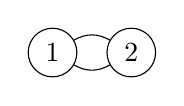
\begin{tikzpicture}
    \node[draw,circle,minimum size=0.2cm] (1) at (-0.5,0) {1};
    \node[draw,circle,minimum size=0.2cm] (2) at (0.5,0) {2};
    \draw[-] (1) to [out=30,in=150] (2);
    \draw[-] (1) to [out=-30,in=-150] (2);
\end{tikzpicture}
& $fxx$ \\

2 & 2 &
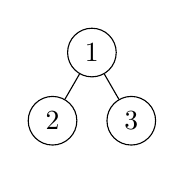
\begin{tikzpicture}
    \node[draw,circle,minimum size=0.2cm] (1) at (0,0.866) {1};
    \node[draw,circle,minimum size=0.2cm] (2) at (-0.5,0) {2};
    \node[draw,circle,minimum size=0.2cm] (3) at (0.5,0) {3};
    \draw[-] (1) to (2);
    \draw[-] (1) to (3);
\end{tikzpicture}
& $fxx$ \\

3 & 3 &
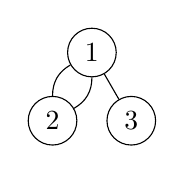
\begin{tikzpicture}
    \node[draw,circle,minimum size=0.2cm] (1) at (0,0.866) {1};
    \node[draw,circle,minimum size=0.2cm] (2) at (-0.5,0) {2};
    \node[draw,circle,minimum size=0.2cm] (3) at (0.5,0) {3};
    \draw[-] (1) to [out=-150,in=90] (2);
    \draw[-] (1) to [out=-90,in=30] (2);
    \draw[-] (1) to (3);
\end{tikzpicture}
& $fxx$ \\

3 & 4 &
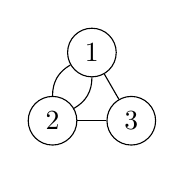
\begin{tikzpicture}
    \node[draw,circle,minimum size=0.2cm] (1) at (0,0.866) {1};
    \node[draw,circle,minimum size=0.2cm] (2) at (-0.5,0) {2};
    \node[draw,circle,minimum size=0.2cm] (3) at (0.5,0) {3};
    \draw[-] (1) to [out=-150,in=90] (2);
    \draw[-] (1) to [out=-90,in=30] (2);
    \draw[-] (1) to (3);
    \draw[-] (2) to (3);
\end{tikzpicture}
& $fxx$ \\

%=====
3 & 3 &
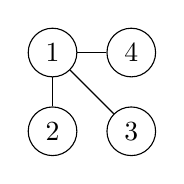
\begin{tikzpicture}
    \node[draw,circle,minimum size=0.2cm] (1) at (0,1) {1};
    \node[draw,circle,minimum size=0.2cm] (2) at (0,0) {2};
    \node[draw,circle,minimum size=0.2cm] (3) at (1,0) {3};
    \node[draw,circle,minimum size=0.2cm] (4) at (1,1) {4};
    \draw[-] (1) to (2);
    \draw[-] (1) to (3);
    \draw[-] (1) to (4);
\end{tikzpicture}
& $fxx$ \\

3 & 4 &
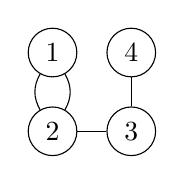
\begin{tikzpicture}
    \node[draw,circle,minimum size=0.2cm] (1) at (0,1) {1};
    \node[draw,circle,minimum size=0.2cm] (2) at (0,0) {2};
    \node[draw,circle,minimum size=0.2cm] (3) at (1,0) {3};
    \node[draw,circle,minimum size=0.2cm] (4) at (1,1) {4};
    \draw[-] (1) to [out=-120,in=120] (2);
    \draw[-] (1) to [out=-60,in=60] (2);
    \draw[-] (2) to (3);
    \draw[-] (3) to (4);
\end{tikzpicture}
& $fxx$ \\

2 & 4 &
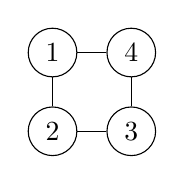
\begin{tikzpicture}
    \node[draw,circle,minimum size=0.2cm] (1) at (0,1) {1};
    \node[draw,circle,minimum size=0.2cm] (2) at (0,0) {2};
    \node[draw,circle,minimum size=0.2cm] (3) at (1,0) {3};
    \node[draw,circle,minimum size=0.2cm] (4) at (1,1) {4};
    \draw[-] (1) to (2);
    \draw[-] (2) to (3);
    \draw[-] (3) to (4);
    \draw[-] (4) to (1);
\end{tikzpicture}
& $fxx$ \\

3 & 4 &
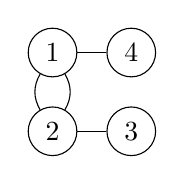
\begin{tikzpicture}
    \node[draw,circle,minimum size=0.2cm] (1) at (0,1) {1};
    \node[draw,circle,minimum size=0.2cm] (2) at (0,0) {2};
    \node[draw,circle,minimum size=0.2cm] (3) at (1,0) {3};
    \node[draw,circle,minimum size=0.2cm] (4) at (1,1) {4};
    \draw[-] (1) to [out=-120,in=120] (2);
    \draw[-] (1) to [out=-60,in=60] (2);
    \draw[-] (2) to (3);
    \draw[-] (1) to (4);
\end{tikzpicture}
& $fxx$ \\

% =========
2 & 4 &
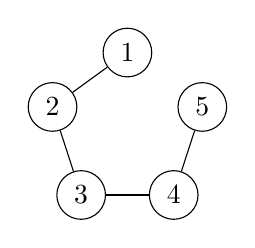
\begin{tikzpicture}
    \node[draw,circle,minimum size=0.2cm] (1) at (0,1) {1};
    \node[draw,circle,minimum size=0.2cm] (2) at (-0.9511,0.3090) {2};
    \node[draw,circle,minimum size=0.2cm] (3) at (-0.5878,-.8090) {3};
    \node[draw,circle,minimum size=0.2cm] (4) at (0.5878,-.8090) {4};
    \node[draw,circle,minimum size=0.2cm] (5) at (0.9511,0.3090) {5};
    \draw[-] (1) to (2);
    \draw[-] (2) to (3);
    \draw[-] (3) to (4);
    \draw[-] (4) to (5);
\end{tikzpicture}
& $fxx$ \\

3 & 4 &
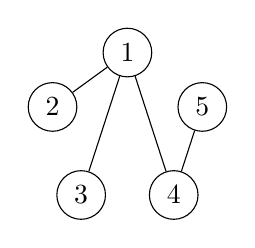
\begin{tikzpicture}
    \node[draw,circle,minimum size=0.2cm] (1) at (0,1) {1};
    \node[draw,circle,minimum size=0.2cm] (2) at (-0.9511,0.3090) {2};
    \node[draw,circle,minimum size=0.2cm] (3) at (-0.5878,-.8090) {3};
    \node[draw,circle,minimum size=0.2cm] (4) at (0.5878,-.8090) {4};
    \node[draw,circle,minimum size=0.2cm] (5) at (0.9511,0.3090) {5};
    \draw[-] (1) to (2);
    \draw[-] (1) to (3);
    \draw[-] (1) to (4);
    \draw[-] (4) to (5);
\end{tikzpicture}
& $fxx$ \\

4 & 4 &
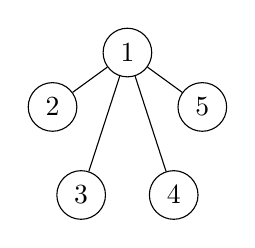
\begin{tikzpicture}
    \node[draw,circle,minimum size=0.2cm] (1) at (0,1) {1};
    \node[draw,circle,minimum size=0.2cm] (2) at (-0.9511,0.3090) {2};
    \node[draw,circle,minimum size=0.2cm] (3) at (-0.5878,-.8090) {3};
    \node[draw,circle,minimum size=0.2cm] (4) at (0.5878,-.8090) {4};
    \node[draw,circle,minimum size=0.2cm] (5) at (0.9511,0.3090) {5};
    \draw[-] (1) to (2);
    \draw[-] (1) to (3);
    \draw[-] (1) to (4);
    \draw[-] (1) to (5);
\end{tikzpicture}
& $fxx$ \\
\end{tabular}

Discussion of singularities. 

And then a list of explicit invariants by group.

And the signatures.

\section{Differential invariants through moving frames}

\todo[inline]{Intro to model bit above. Steal equations from dispaper. TBC}
Cartan developed the moving frame to compute invariants.

Then computations.

Then the graphs and the weights.

And then a list of explicit invariants by group.

And the signatures.

\section{Extension to larger groups, role of colour, etc.}

\todo[inline]{Largely discursive? Except conformal.}

\section{Use in practice; noise, singularities}
 \todo[inline]{Experimental}

\section{Algorithms}
 This will go in paper 2, but let's start in here.

\todo[inline]{Pseudocode for the matlab experimental code}
\todo[inline]{Something about computing transvectants?}


\section{Experiments}

\todo[inline]{Signature examples}
\todo[inline]{Noise}
\todo[inline]{Spot the group}
\todo[inline]{Example on bits of images}

\end{document}
